

\section{Effect on an electric guitar}
In order to give an electrical guitar effect, all commently used effect needs to be analysed. This section aims is to give a overview of all frequently used guitar effect. These effect is: 

\begin{itemize}
 \item Equalizing
 \item Reverberation
 \item Overdrive
 \item Distortion
 \item Chorus
 \item Flanger
 \item Wah-Wah
\end{itemize}

To give an owerviwe how the effect influence the sound, all effect is descriped below

\newpage

\input{chapters/analysing/equalizing}\label{sec:equalizing} 
\subsection{Delay}
Delay is an audio effect which memorizes the input signal for a customized time, and then release it without changing anything else than the amplitude. The delayed signal can either be played back multiple times or only once . When the signal is delayed and then played back multiple times, it can either be amplified or attenuated. If the delayed signal is amplified, it will start to oscillate. If the wanted effect is an echo, the delayed signal shouldn't be kept alive, then the gain in the feedback must be reduced in order to attenuate the signal.  \autoref{fig:delay_block} shows a block diagram of a simple delay, "echo" unit.


\begin{figure} [htbp]
 \centering
\begin{picture}(0,0)%
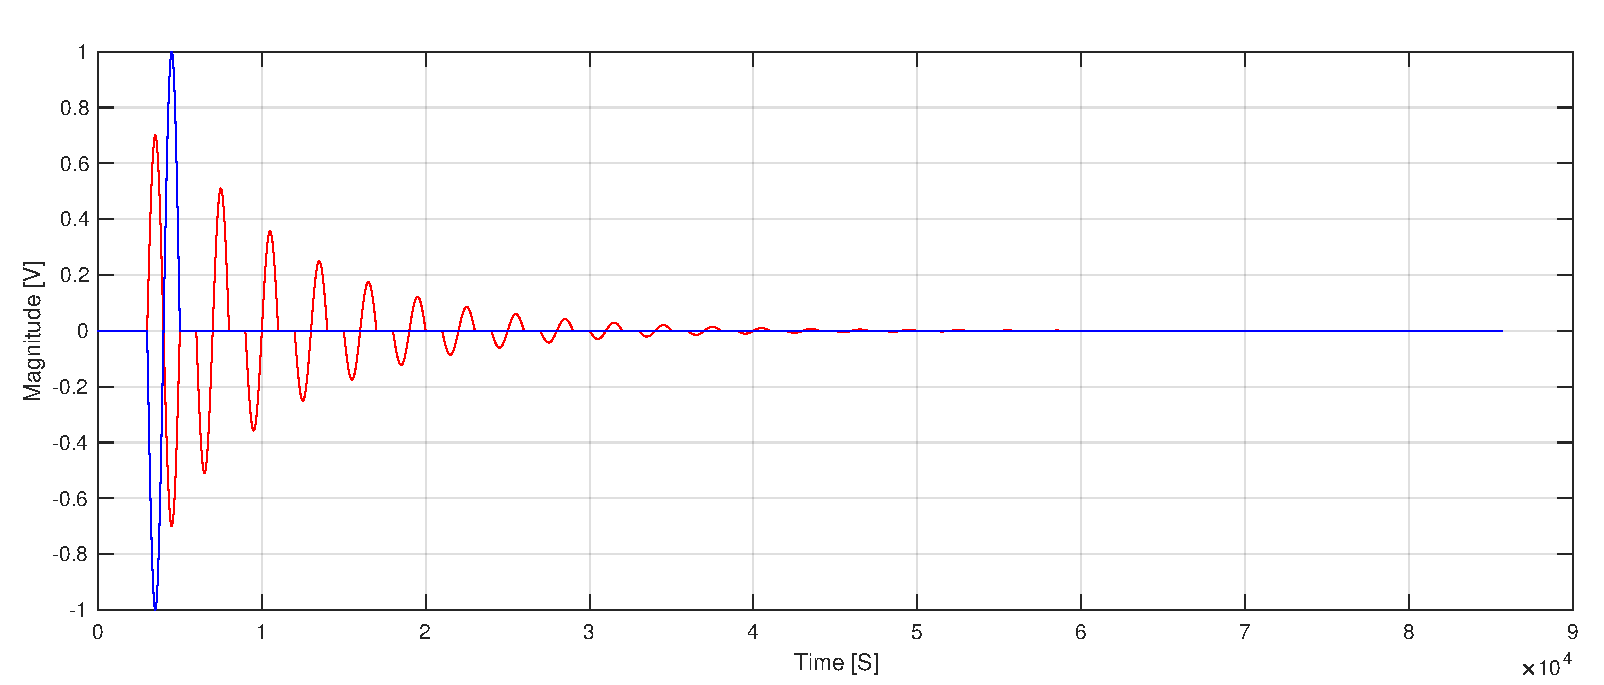
\includegraphics{delay.pdf}%
\end{picture}%
\setlength{\unitlength}{4144sp}%
%
\begingroup\makeatletter\ifx\SetFigFont\undefined%
\gdef\SetFigFont#1#2#3#4#5{%
	\reset@font\fontsize{#1}{#2pt}%
	\fontfamily{#3}\fontseries{#4}\fontshape{#5}%
	\selectfont}%
\fi\endgroup%
\begin{picture}(5035,1329)(1491,-118)
\put(4726,704){$Gain$}%

\put(3106,479){$Delay$}%

\put(5814,672){$Output$}%

\put(1506,659){$Input$}%

\end{picture}%

  \caption{The photo shows a block diagram on a delay unit \citep{delay_block}}
  \label{fig:delay_block}
\end{figure}

The block diagram \autoref{fig:delay_block} shows a delay unit with a feedback line that has an adjustable gain. The feedback signal is either attenuated or amplified depending on the gain value and then added to the delay line input \cite{delay_echo}. The following \autoref{fig:delay_echo} shows the effect in time domain.

\begin{figure} [htbp]
 \centering
  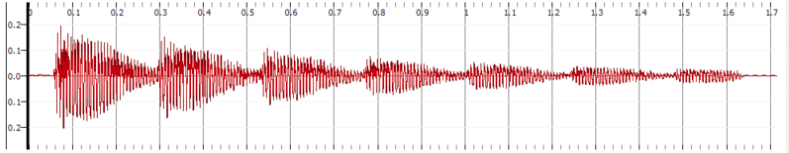
\includegraphics[width=1\textwidth]{delay_echo}
  \caption{The photo shows a echo in time domain}
  \label{fig:delay_echo}
\end{figure}
\todo[inline]{make figure i matlab}

The \autoref{fig:delay_echo} shows that the main signal is repeated and attenuated 6 time before it is totally attenuated. A time domain diagram is shown at \autoref{fig:delay_timed}.

\begin{figure} [htbp]
 \centering
\begin{picture}(0,0)%
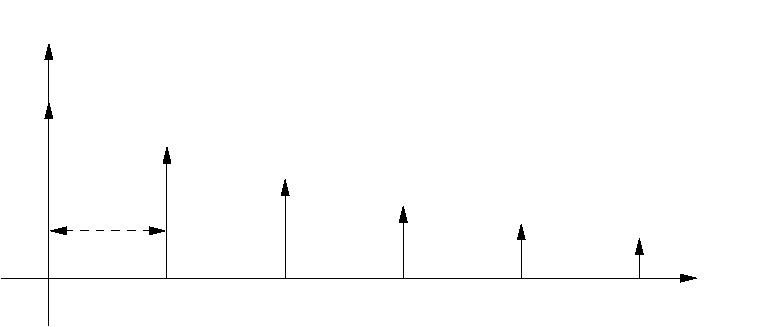
\includegraphics{delay_timed.pdf}%
\end{picture}%
\setlength{\unitlength}{4144sp}%
%
\begingroup\makeatletter\ifx\SetFigFont\undefined%
\gdef\SetFigFont#1#2#3#4#5{%
  \reset@font\fontsize{#1}{#2pt}%
  \fontfamily{#3}\fontseries{#4}\fontshape{#5}%
  \selectfont}%
\fi\endgroup%
\begin{picture}(5843,2478)(4129,-5833)
\put(9496,-5506){$Time$}%
\put(4231,-3526){$Magnitude$}%
\put(4591,-4291){$Main$}%
\put(5536,-4606){$G$}%
\put(6436,-4876){$G^2$}%
\put(7336,-5056){$G^3$}%
\put(8236,-5191){$G^4$}%
\put(9136,-5281){$G^5$}%
\put(4861,-5056){$t\Delta$}%
\put(6256,-5776){$t2$}%
\put(5356,-5776){$t1$}%
\put(7156,-5776){$t4$}%
\put(8056,-5776){$t5$}%
\put(8956,-5776){$t6$}%
\end{picture}%
  \caption{The figure shows the impulse respond of the delay unit}
  \label{fig:delay_timed}
\end{figure}
\label{sec:delay} 
\section{Reverberation}
Reverberation is \label{sec:reverberation} 
\subsection{Overdrive and Distortion} 

The distortion effects changes the sound of the played instrument by increasing the gain. It is commonly used the with the electric guitar. The sound changes due to the clipping effect. \\
\todo[inline]{Muhammed: "It is commonly used in the with the electric guitar" does something missing?}

The clipping effect is a way of changing the waveform when an amplifier is over driven; forcing it to deliver an output that is higher than its maximum capability. \\
The part of the waveform where the amplifier is asked to get a value higher than its maximum capacity gets the maximum value the amplifier can give. It means that all the parts of the waveform where the amplifier is pushed more than its capacity will have the same amplitude. The signal is then 'clipped'. An illustration of this effect is shown in \autoref{fig:clipping1}.\\

\begin{figure} [htbp]
	\centering
  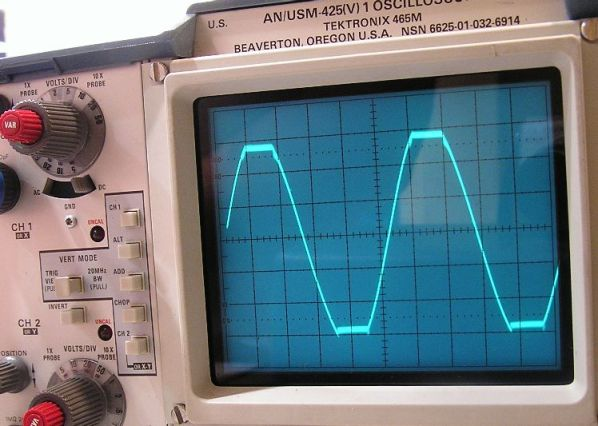
\includegraphics[width=0.7\textwidth]{clippingeffect.jpg}
  \caption{Photo showing the effect of clipping, a consequence of the overdrive or distortion effect.}
  \label{fig:clipping1}
\end{figure}


The consequences in the frequency domain are that the clipping effect creates more harmonics at high frequency than the signal without the clipping effect. \\

The clipping effect in signal processing happens when the amplitude is limited by a number and if during the processing the amplitude surpasses this limit, clipping happens because the value is then maxed to the maximum number that can be handled digitally. The maximum amplitude that can be handled is determined by the number of bits the system uses. The maximum number for a \SI{16}{\bit}  signed integers system is $\frac{2^{16}}{2} = \SI{32768}{\cdot}$ which means that if a value has an amplitude higher than this number the clipping effect occurs. \\

In any clipping technique, there is a creation of new harmonics. In the case of soft clipping, the new harmonics are multiples of the harmonics of the original tone. Valve Overdrive is a soft clipping technique for instance. In the case of hard clipping, they are not multiples which results to what is called intermodulation. Hard clipping usually happens when the harmonics of the original signal are not related by a multiple. Transistor overdrive is an example of hard clipping.  Effects of hard and soft clipping on the waveforms are shown in \autoref{fig:clipping2}.

In the previous paragraphs, distortion and overdrive has been explained as if they are the same effects. In fact, there is a small difference between the two. Distortion changes the original tone more than overdrive which means that distortion will generate more extra harmonics than overdrive and their amplitude tend to be higher. Overdrive effect has "cleaner" consequences on the final tone than distortion. Overdrive is often assigned to soft clipping while distortion is assigned to hard clipping.

\begin{figure} [htbp]
	\centering
  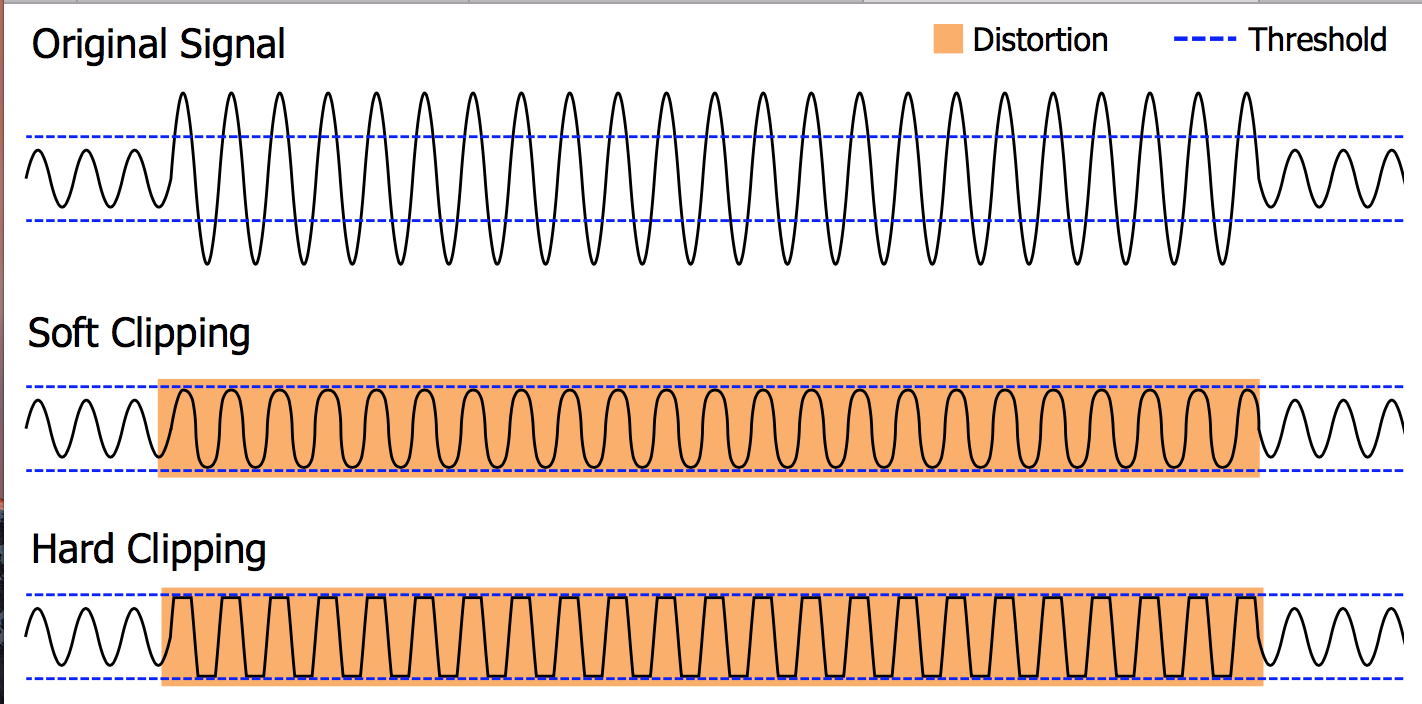
\includegraphics[width=0.7\textwidth]{softhardclipping.png}
  \caption{Photo showing the effect of hard and soft clipping, a consequence of the overdrive or distortion effect.}
  \label{fig:clipping2}
\end{figure}


\label{sec:overdrive} 
\subsection{Chorus and Flanger Effect} \label{sec:chorus} 

%\label{chor_flang}

The chorus effect is obtained when a signal is delayed and then mixed with its original version \citep{chorus_gibson} \citep{chorus_apple}. \\
The chorus effect takes a single audio signal as input and applies different delay values to it. Chorus effect using one delay is called flanger. Each of the delayed signals are then mixed with the original audio input. \\
A \gls{lfo} can be used to make the delay times vary. Different \gls{lfo}s can be used for each of the delay channels to make a richer sound mix and avoiding repetitive sound but it implies more computations. The same \gls{lfo} can be used for all the delay channels but not at the same cycle for each delay \citep{chorus_testtone}. \\ 

Different parameters on the chorus effect can changed by settings on the hardware. Some of these are:\\
\begin{itemize}
\item \textbf{Delay time}: The time difference between the original sound and the delayed one (The frequency of the signal from the \gls{lfo}).
\item \textbf{Chorus size}: The number of delayed sounds that will be mixed.
\item \textbf{Depth}: The amplitude of the signal from the \gls{lfo}.
\item \textbf{Waveform}: The waveform of the signal from the \gls{lfo} can be changed to triangle, sine, log ect. \citep{hobby_hour_chorus}
\item \textbf{Gain}: The amplification of the delayed signal.
\end{itemize} \citep{chorus_parameters}

A block diagram for  the chorus and flanger effect is shown in \autoref{fig:chorus_diag}.

\begin{figure} [htbp!]
	\centering
\begin{picture}(0,0)%
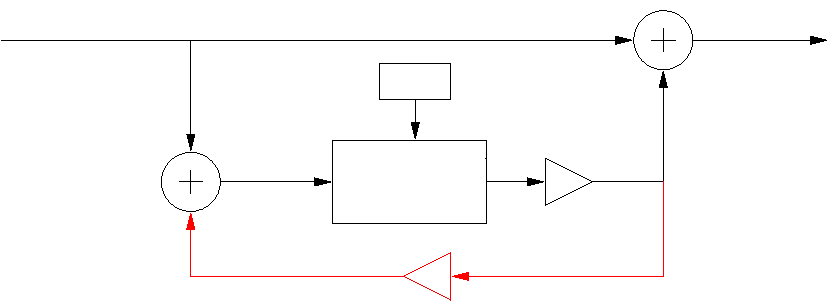
\includegraphics{chorus_diag.pdf}%
\end{picture}%
\setlength{\unitlength}{4144sp}%
%
\begingroup\makeatletter\ifx\SetFigFont\undefined%
\gdef\SetFigFont#1#2#3#4#5{%
	\reset@font\fontsize{#1}{#2pt}%
	\fontfamily{#3}\fontseries{#4}\fontshape{#5}%
	\selectfont}%
\fi\endgroup%
\begin{picture}(6327,3018)(3766,-3493)
\put(6706,-1366){\color[rgb]{0,0,0}LFO}%

\put(8101,-1636){\color[rgb]{0,0,0}Gain}%

\put(3781,-646){\color[rgb]{0,0,0}Input}%

\put(9406,-646){\color[rgb]{0,0,0}Output}%

\put(6571,-1906){\color[rgb]{0,0,0}Delay}%

\put(6616,-3211){\color[rgb]{1,0,0}Delay}%

\put(8101,-2986){\color[rgb]{1,0,0}Gain}%

\put(6706,-2671){\color[rgb]{1,0,0}LFO}%

\end{picture}%



\caption{Block Diagram of the chorus effect.}
\label{fig:chorus_diag}
\end{figure}


As it can be seen on the block diagram in figure \autoref{fig:chorus_diag}, a signal that hasn't been affected by any changes is added to the same signal delayed, controlled by the \gls{lfo}. The addition is done just before the output. The chorus effect is represented by the black and the red parts of the block diagram. The flanger effect is represented only by the black parts of the block diagram. In \autoref{fig:chorus_and_flanger_time} the impulse response of the chorus and the flanger effect are shown. Its is seen that with a pulse as the input, in the flanger effect, the output will be the original pulse, followed by an echo. The period before this echo arrives varies, based on the \gls{lfo}. When using the chorus effect several echoes will arrive, still with varying delay time. 

\begin{figure}[htbp!]
\centering
\def\svgwidth{\columnwidth}
\scalebox{0.8}{\input{figures/analysing/chorus_and_flanger_time_domain.pdf_tex}}
\caption{Impulse response of the flanger effect (black) and the chorus effect (red).}
		\label{fig:chorus_and_flanger_time}
\end{figure}










\label{sec:chorus} 
\subsection{Wah-Wah}\label{sec:wah-wah} 

The effect takes the original signal and mix it with another signal that passes through a bandpass filter. The bandpass filter is time varying, which means that it changes its position in the frequency spectrum \citep{wah-wah_course}. \\
The automatic Wah-Wah effect have some different parameters that can be changed to customize the effect:\\

\begin{itemize}
	\item \textbf{The \gls{lfo} frequency}: it sets the speed at which the bandpass filter moves in the frequency spectrum.
	\item \textbf{\gls{lfo} start phase}: Determine where should the bandpass filter start.
	\item \textbf{\gls{lfo} depth}: the range of frequencies it should work on, high depth gives a bigger range and vice versa.
\end{itemize} \citep{wah-wah_audacity}

A block diagram of the effect is illustrated in \autoref{fig:wah_diag}.  

\begin{figure} [htbp]
	\centering
\begin{picture}(0,0)%
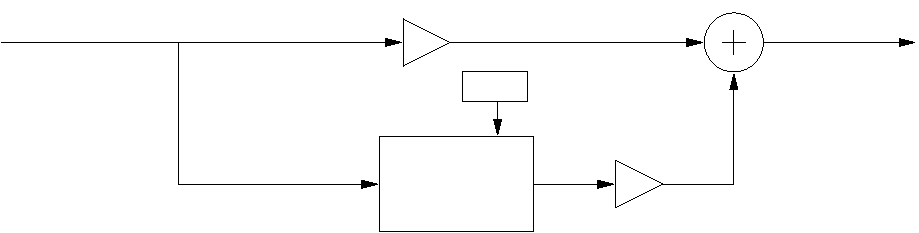
\includegraphics{wah_diag.pdf}%
\end{picture}%
\setlength{\unitlength}{4144sp}%
%
\begingroup\makeatletter\ifx\SetFigFont\undefined%
\gdef\SetFigFont#1#2#3#4#5{%
  \reset@font\fontsize{#1}{#2pt}%
  \fontfamily{#3}\fontseries{#4}\fontshape{#5}%
  \selectfont}%
\fi\endgroup%
\begin{picture}(6999,1770)(2689,-2233)
\put(6841,-1591){\textit{Wah-Wah Gain}}%
\put(5626,-2041){$Filter$}%
\put(6136,-1186){\textit{LFO or Pedal}}%
\put(2746,-646){$Input$}%
\put(8686,-646){$Output$}%
\put(5626,-1816){$Bandpass-$}%
\put(5986,-646){$Gain$}%
\end{picture}%
	\caption{Block diagram of the wah-wah effect}
	\label{fig:wah_diag}
\end{figure}

It can be seen on the block diagram that the filtered signal is added to the direct signal. Thus, this block diagram is a representation of the wah-wah effect.  \\


The phaser effect can be created by using a band-stop filter instead of a bandpass filter using the same block diagram presented in \autoref{fig:wah_diag} \citep{wah-wah_cardiff}. \\

There is another type of wah-wah effect called M-fold wah-wah which uses multiple M-tap bandpass filters that move around the spectrum at the same time \citep{wah-wah_cardiff}. \\

An example of a time domain response is shown in figure \autoref{fig:wah-wah-response}. \\

\begin{figure} [htbp!]
	\centering
	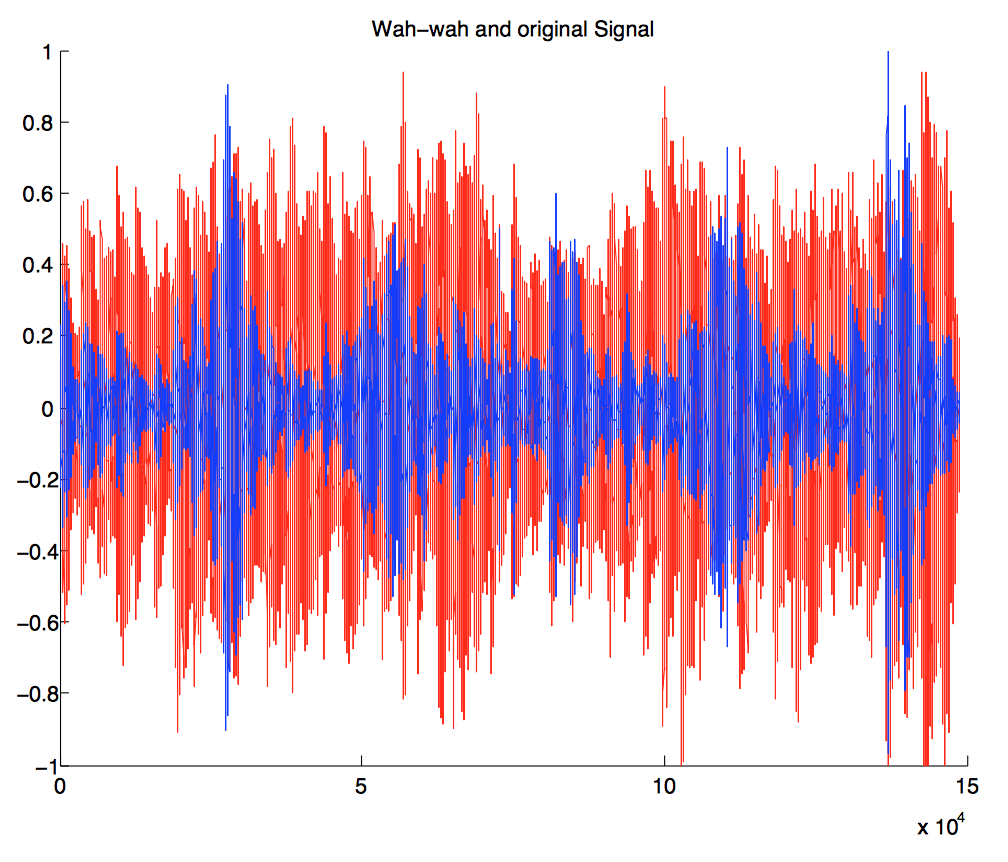
\includegraphics[width=0.6\textwidth]{wah-wah-response.png}
	\caption{Time domain response of the original sound (red) and the one after having the wah-wah effect (blue) \citep{wah-wah_cardiff}.}
	\label{fig:wah-wah-response}
\end{figure}
\todo[inline]{write about wah wah frequency in text}

\todo[inline]{Jonas: Muhammed, can you explain the above time domain spectra?(and the block diagram)}
\todo[inline]{Sebastian: Maybe make figure our self, because axis descriptions are missing now}

As it can be seen on \autoref{fig:wah-wah-response}, the wah-wah effect reduced the amplitudes of many parts of the wave-form compared to the signal without the wah-wah effect. Some of the them remained the same. It is due to the bandpass-filtering.
In \autoref{fig:wah_wah_frequency} an illustration of the bandpass filter in the wah-wah effect in frequency domain is shown. 

\begin{figure}
\centering
\def\svgwidth{\columnwidth}
\input{figures/analysing/wah_wah_frequency_domain.pdf_tex}
\caption{Frequency domain illustration of bandpass filter in the wah-wah effect}
		\label{fig:wah_wah_frequency}
\end{figure}

It is shown that the bandpass filter can be moved in frequency. This movement is done either by an \gls{lfo} or with an expression pedal.
\label{sec:wah-wah} 
